\subsection{Diseños preliminares}

Empezamos exponiendo algunos diseños preliminares que surgieron cuando empezábamos 
con el trabajo. Los mismos también sirven para dar un panorama de la evolución 
que fuimos desarrollando sobre los diseños y las decisiones tomadas. 

Mostramos primero un diagrama de objetos, el cual fue de los primeros que 
planteamos, para tratar de darnos un panorama de cómo queríamos organizar 
el conocimiento y las responsabilidades. 

\subsubsection{Diagrama de objetos de las características físicas del yacimiento en el Simulador}

\begin{figure}[H]
\caption{Diagrama de objetos preliminar}
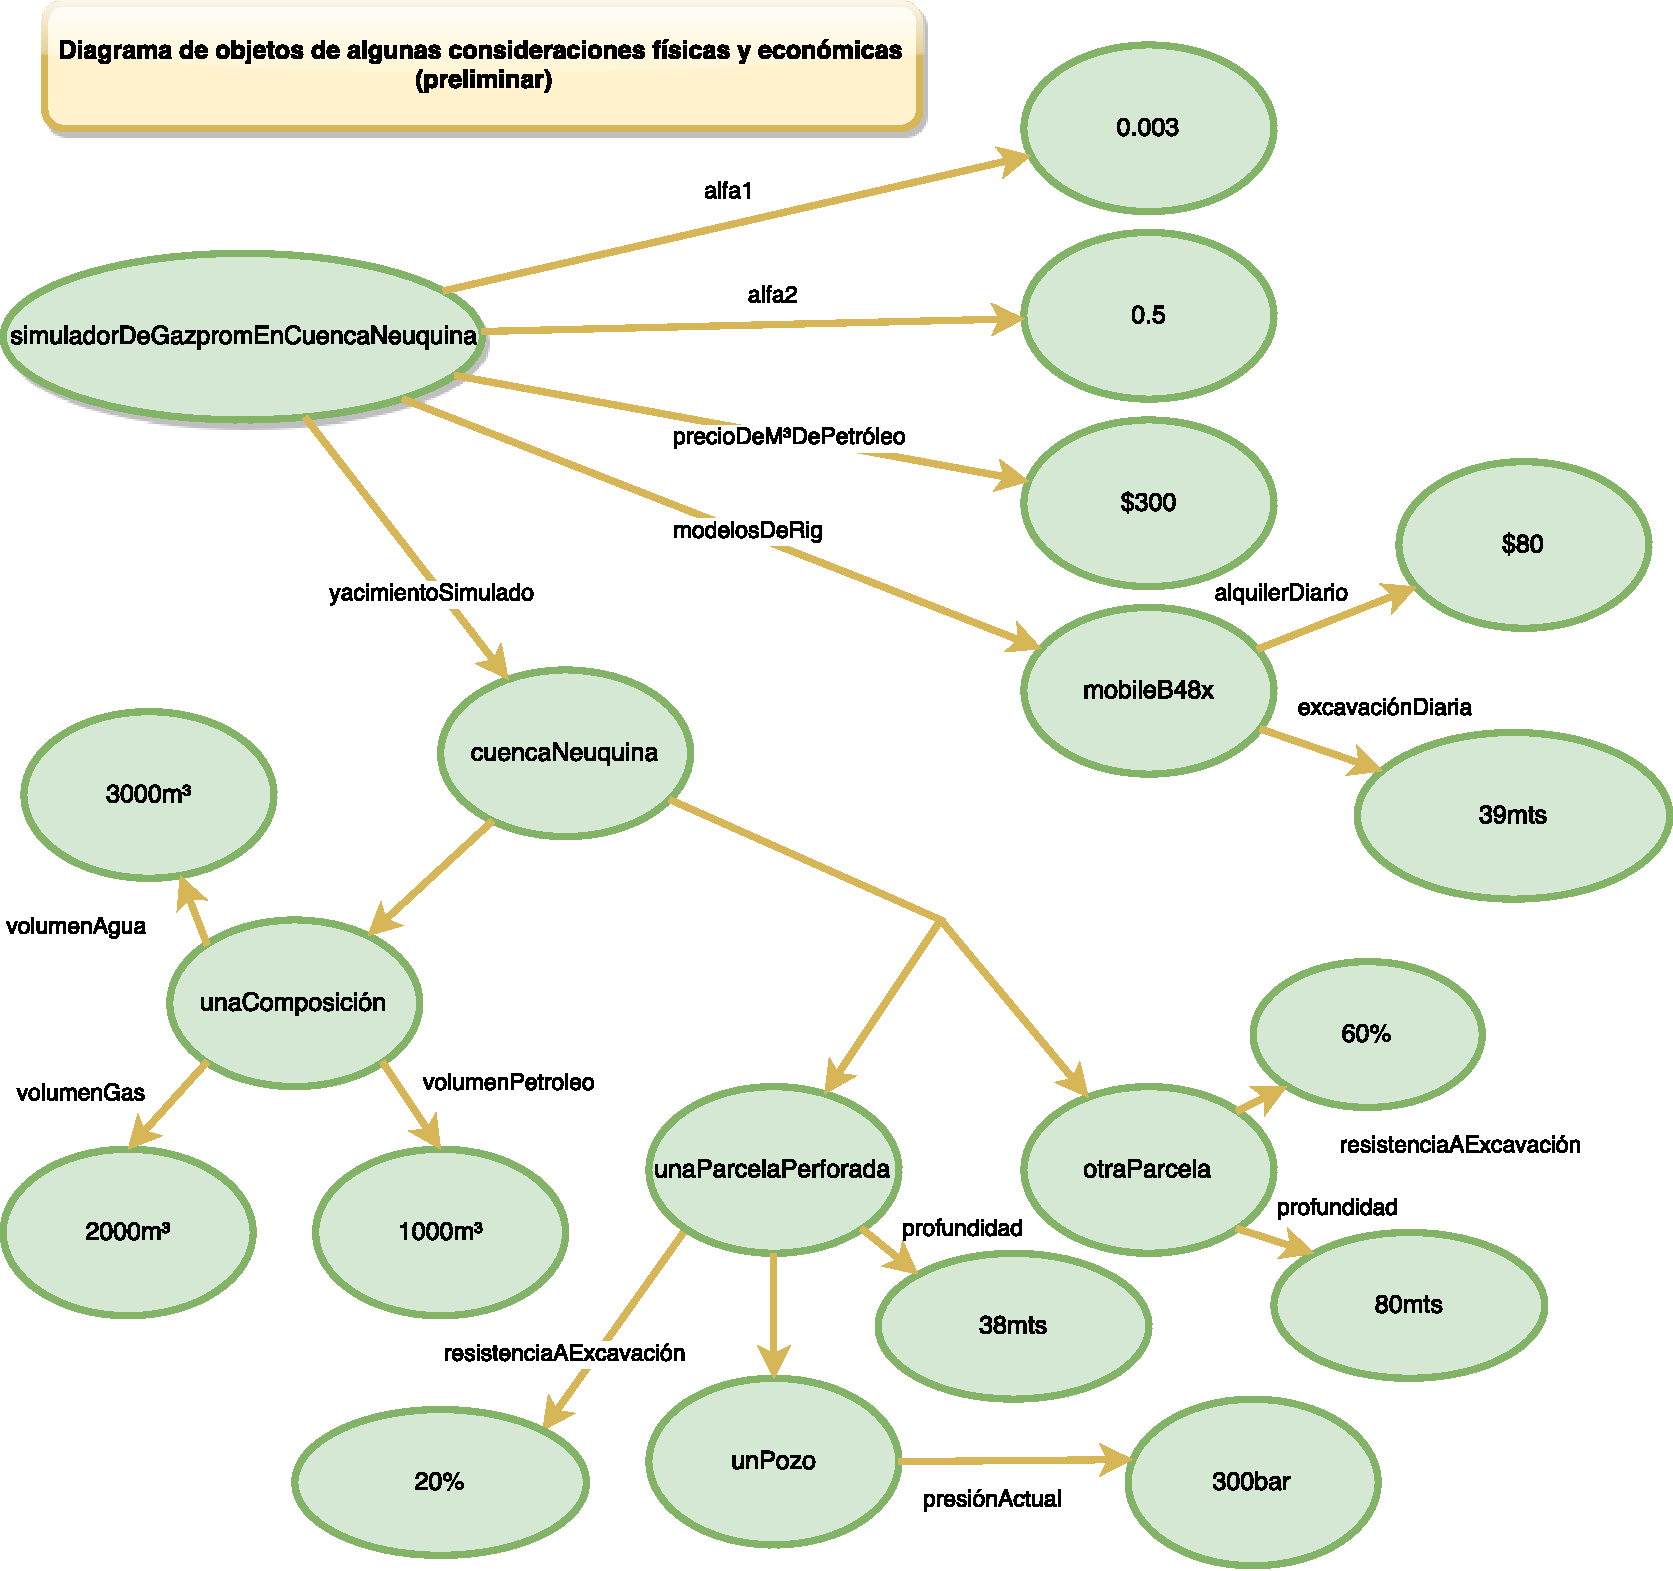
\includegraphics[width=\textwidth, height=\textheight, keepaspectratio]{objetos-modelado-fisico.pdf}
\end{figure}

Por un lado, planteamos que habría un objeto ``central'' que sería el mismo 
objeto que representa al simulador. Éste conocería otros como el objeto de un 
yacimiento, parámetros de configuración, los RIGS que tiene alquilados, plantas 
disponibles, entre otras cosas. Lo que se muestra en el diagrama es una visión 
parcial de la idea que teníamos en ese momento. 

Surgen otras nociones fundamentales, como por ejemplo que un yacimiento debería 
conocer otro objeto que representa la composición del mismo, o que las parcelas 
conocen a sus respectivos pozos en el caso de tener uno. Tratamos de mantener 
lo más posible un isomorfismo con la realidad en esta primera iteración. 

A esta altura sin embargo, y solo con este diagrama, no queda claro cómo es que 
se realizaría la ejecución propiamente dicha de la simulación. Tampoco por qué 
o cómo es que son seleccionadas las parcelas o RIGS para desempeñar tareas. \\

De lo especificado que debe realizar el simulador, se nos dice que es el equipo 
de ingeniería el responsable de tomar estas decisiones, y que lo hará mediante 
la elección de estrategias parametrizables para determinar diferentes criterios. 
Por ejemplo, debe poder elegirse el criterio que determina cuándo se deja de 
explotar un yacimiento, y este podría ser, por ejemplo, luego de una cantidad de 
tiempo fijo, o cuando la composición del yacimiento ya no es rentable. 

Nos surge entonces naturalmente la idea de representar estos \textbf{criterios} 
como objetos en sí mismo en nuestro diseño. A su vez, vemos que vamos a querer 
un diseño flexible respecto a cómo pueden ser estos criterios, porque para un 
criterio podríamos querer tener \textbf{muchas diferentes estrategias} (y además 
no conocemos todas con antelación). \\

Lo que decidimos entonces fue representar a cada tipo de criterio con una clase 
correspondiente, así tendremos la clase de los criterios de corte, la clase de 
los criterios de alquiler de RIGS, y así siguiendo. Además, queremos que quién 
utilice estos criterios (por ahora, el objeto del simulador) pueda abstraerse de 
si la estrategia que está utilizando es una u otra. Lo que vamos a hacer es 
mantener las clases de los criterios como abstractas, implementando una interfaz 
mínima que debe ofrecer ese criterio, y las distintas estrategias serán 
subclases de la misma. Veamos un ejemplo. 

\subsubsection{Diagrama de clases preliminar, criterios de corte}

\begin{figure}[H]
\centering
\caption{Fragmento diagrama de clases preliminar, para criterios de corte}
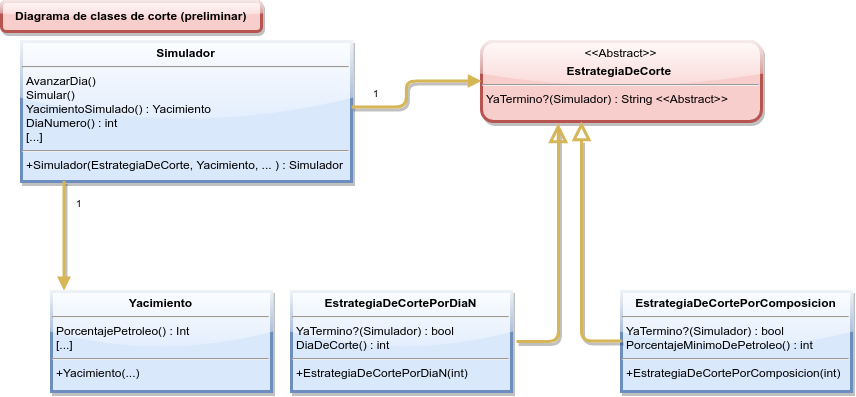
\includegraphics[width=0.95\textwidth, keepaspectratio]{clases-preliminar}
\end{figure}

Aquí puede verse la idea de la que hablábamos recién. En el ejemplo, la idea
es que todas las estrategias de corte sean polimórficas y puedan responder al 
mensaje \texttt{YaTermino?}, el cual le indicará al simulador si debe cortar 
con la simulación o no. Sin embargo éste no necesita saber con qué estrategia 
de corte está tratando. Esto se condice naturalmente con el patrón de diseño 
\textit{strategy} visto en la materia. \\

Mostramos a continuación un par de diagramas de secuencia siguiendo el ejemplo 
de las estrategias de corte, desarrollando cómo podría funcionar cada una. 

\subsubsection{Diagrama de secuencia de las estrategias de corte}

\begin{figure}[H]
\caption{Criterio de corte por cantidad de días, diseño preliminar}
\centering
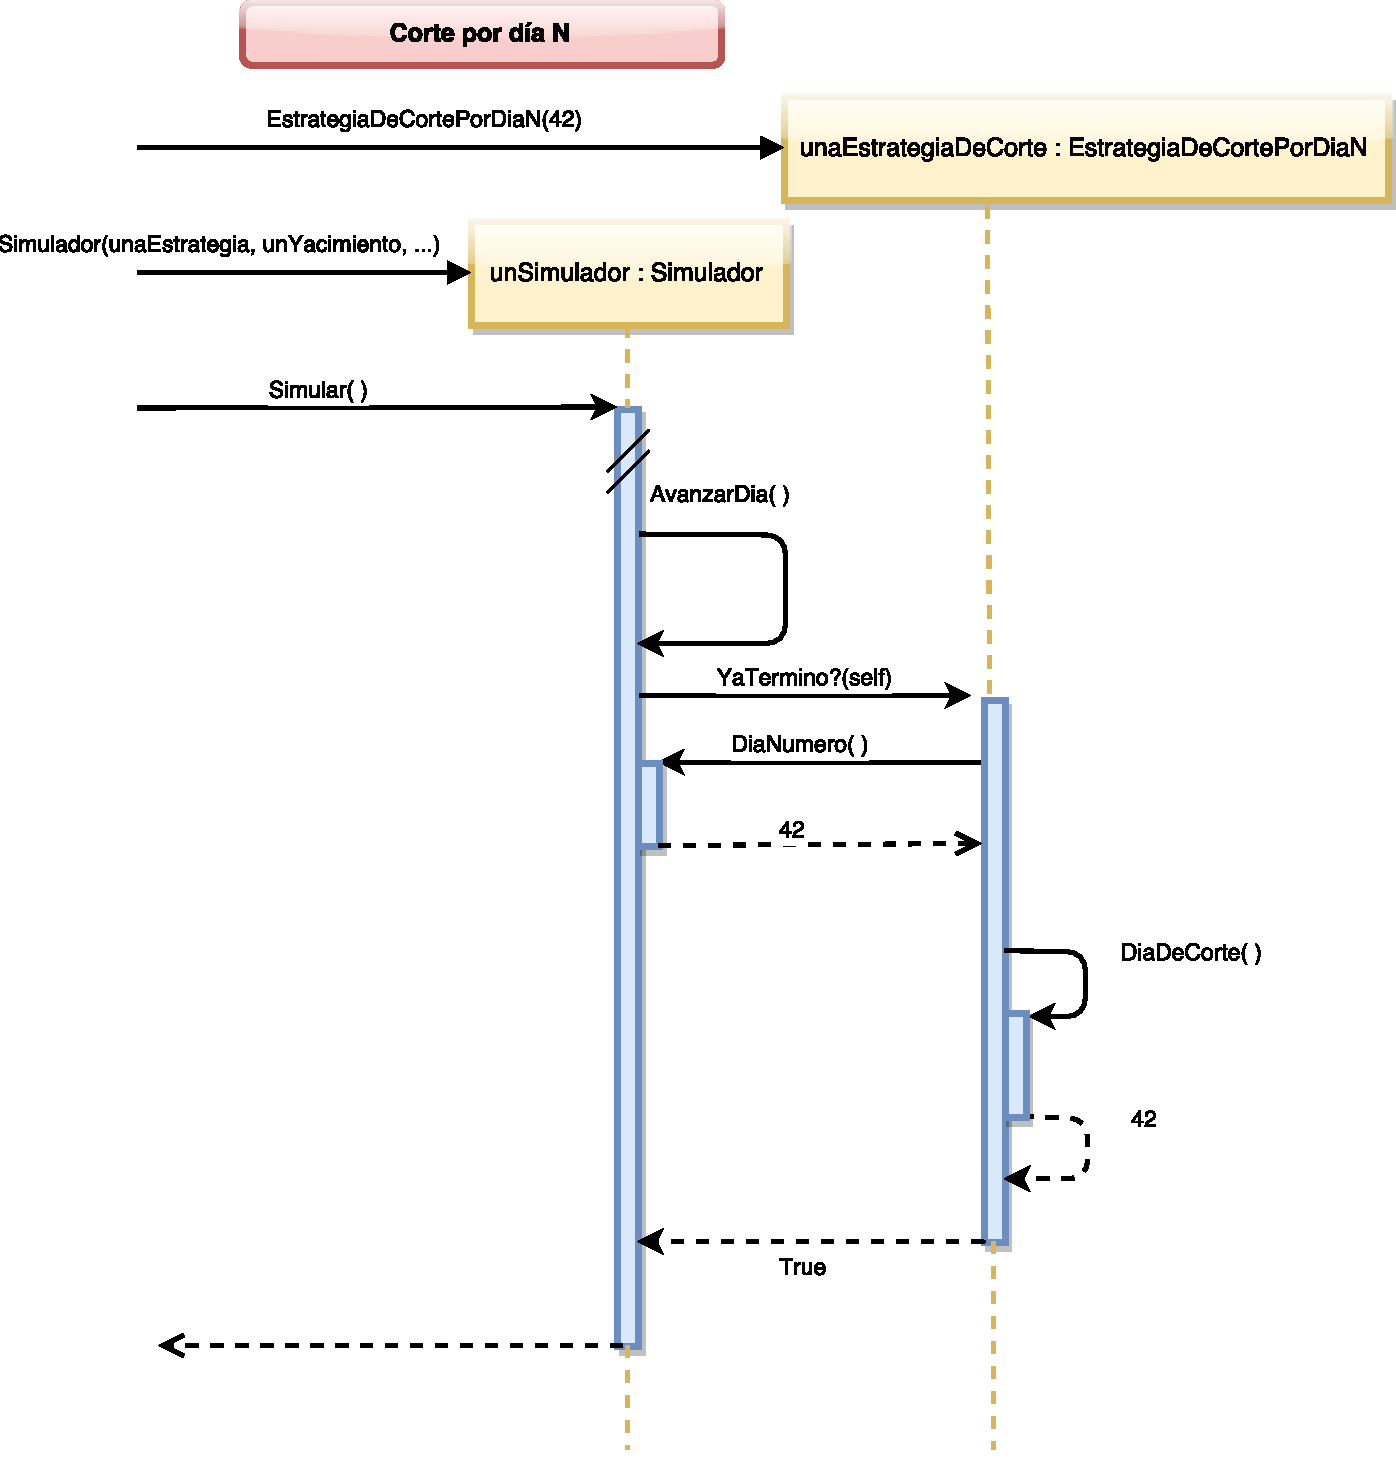
\includegraphics[width=\textwidth, height=\textheight, keepaspectratio]{secuencia-corte-dia.pdf}
\end{figure}

La secuencia comienza con el mensaje \texttt{Simular} del simulador. Éste 
internamente deberá ser responsable de avanzar un día en la simulación, con 
todo lo que eso conlleva, como la extracción de producto como la construcción 
de plantas o tanques. Entre esas, también necesita saber si debe terminar con la 
simulación, para esto le pregunta a su criterio de corte, que en este caso es 
fijo por cantidad de días, mediante el mensaje \texttt{YaTermino?}. El criterio 
de corte a su vez (como pasará con otros criterios) necesita poder conocer 
ciertas cosas del estado actual de la simulación, es por esto que dentro del 
mensaje \texttt{YaTermino?} el simulador en envía a sí mismo como colaborador. 
De esta manera luego el criterio de corte puede preguntarle el simulador 
cuál es el día actual de simulación. Con ese resultado, el criterio hace la 
comparación con su parámetro y devuelve su respuesta binaria. 

\begin{figure}[H]
\caption{Criterio de corte por composición del yacimiento, diseño preliminar}
\centering
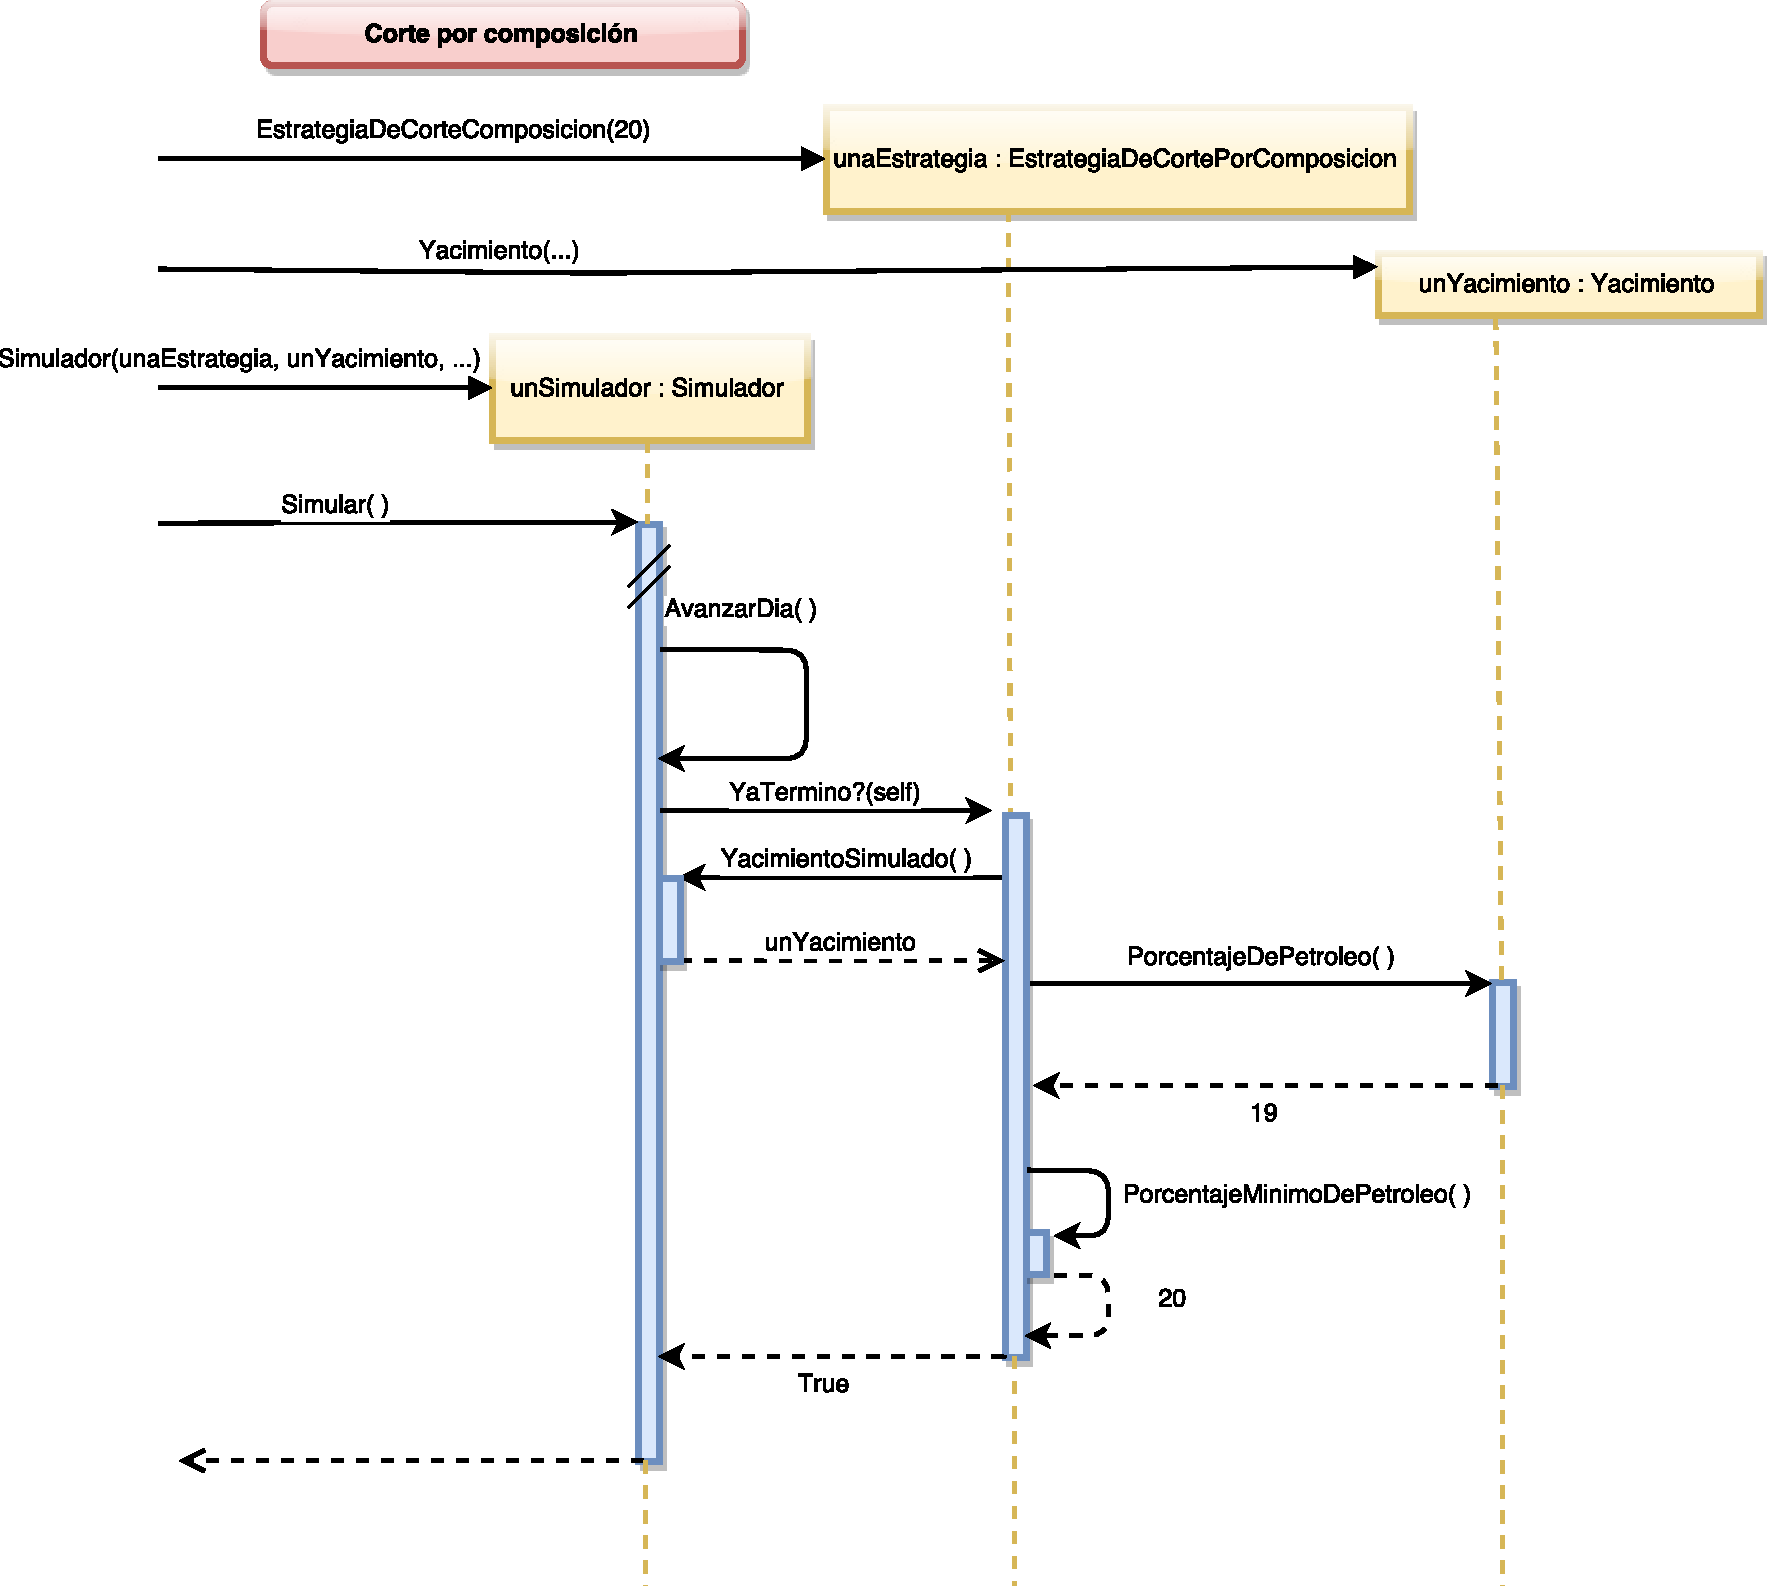
\includegraphics[width=\textwidth, height=\textheight, keepaspectratio]{secuencia-corte-composicion.pdf}
\end{figure}

Este otro diagrama se desarrolla de manera similar. La diferencia surge cuando 
el simulador envía el mensaje \texttt{YaTermino?} a su criterio de corte. 
Nuevamente, el simulador se envía a si mismo como colaborador del mensaje. En 
este caso, el criterio le pide al simulador por su yacimiento, mediante otro 
mensaje. Luego con el yacimiento obtiene la concentración de petróleo que hay en 
el mismo, compara con el valor mínimo aceptable, y devuelve la respuesta binaria. \\

Podemos ver entonces que mediante el uso de este patrón podemos mantener 
polimorfismo entre las diferentes estrategias de un mismo criterio, a la vez 
desacoplando la responsabilidad del simulador de la toma de decisiones del 
equipo de ingeniería. Por esto, decidimos conservar esta idea en lo que siguió 
de nuestra solución, que además fue un eje central para la misma. 

%%%%%%%%%%%%%%%%%%%% FIN? %%%%%%%%%%%%%%%%
